\newpage
\subsubsection{UCS 8 - Report tabellare degli accessi ai luoghi dell'organizzazione}%kite level
\begin{figure}[h!]
	\centering
    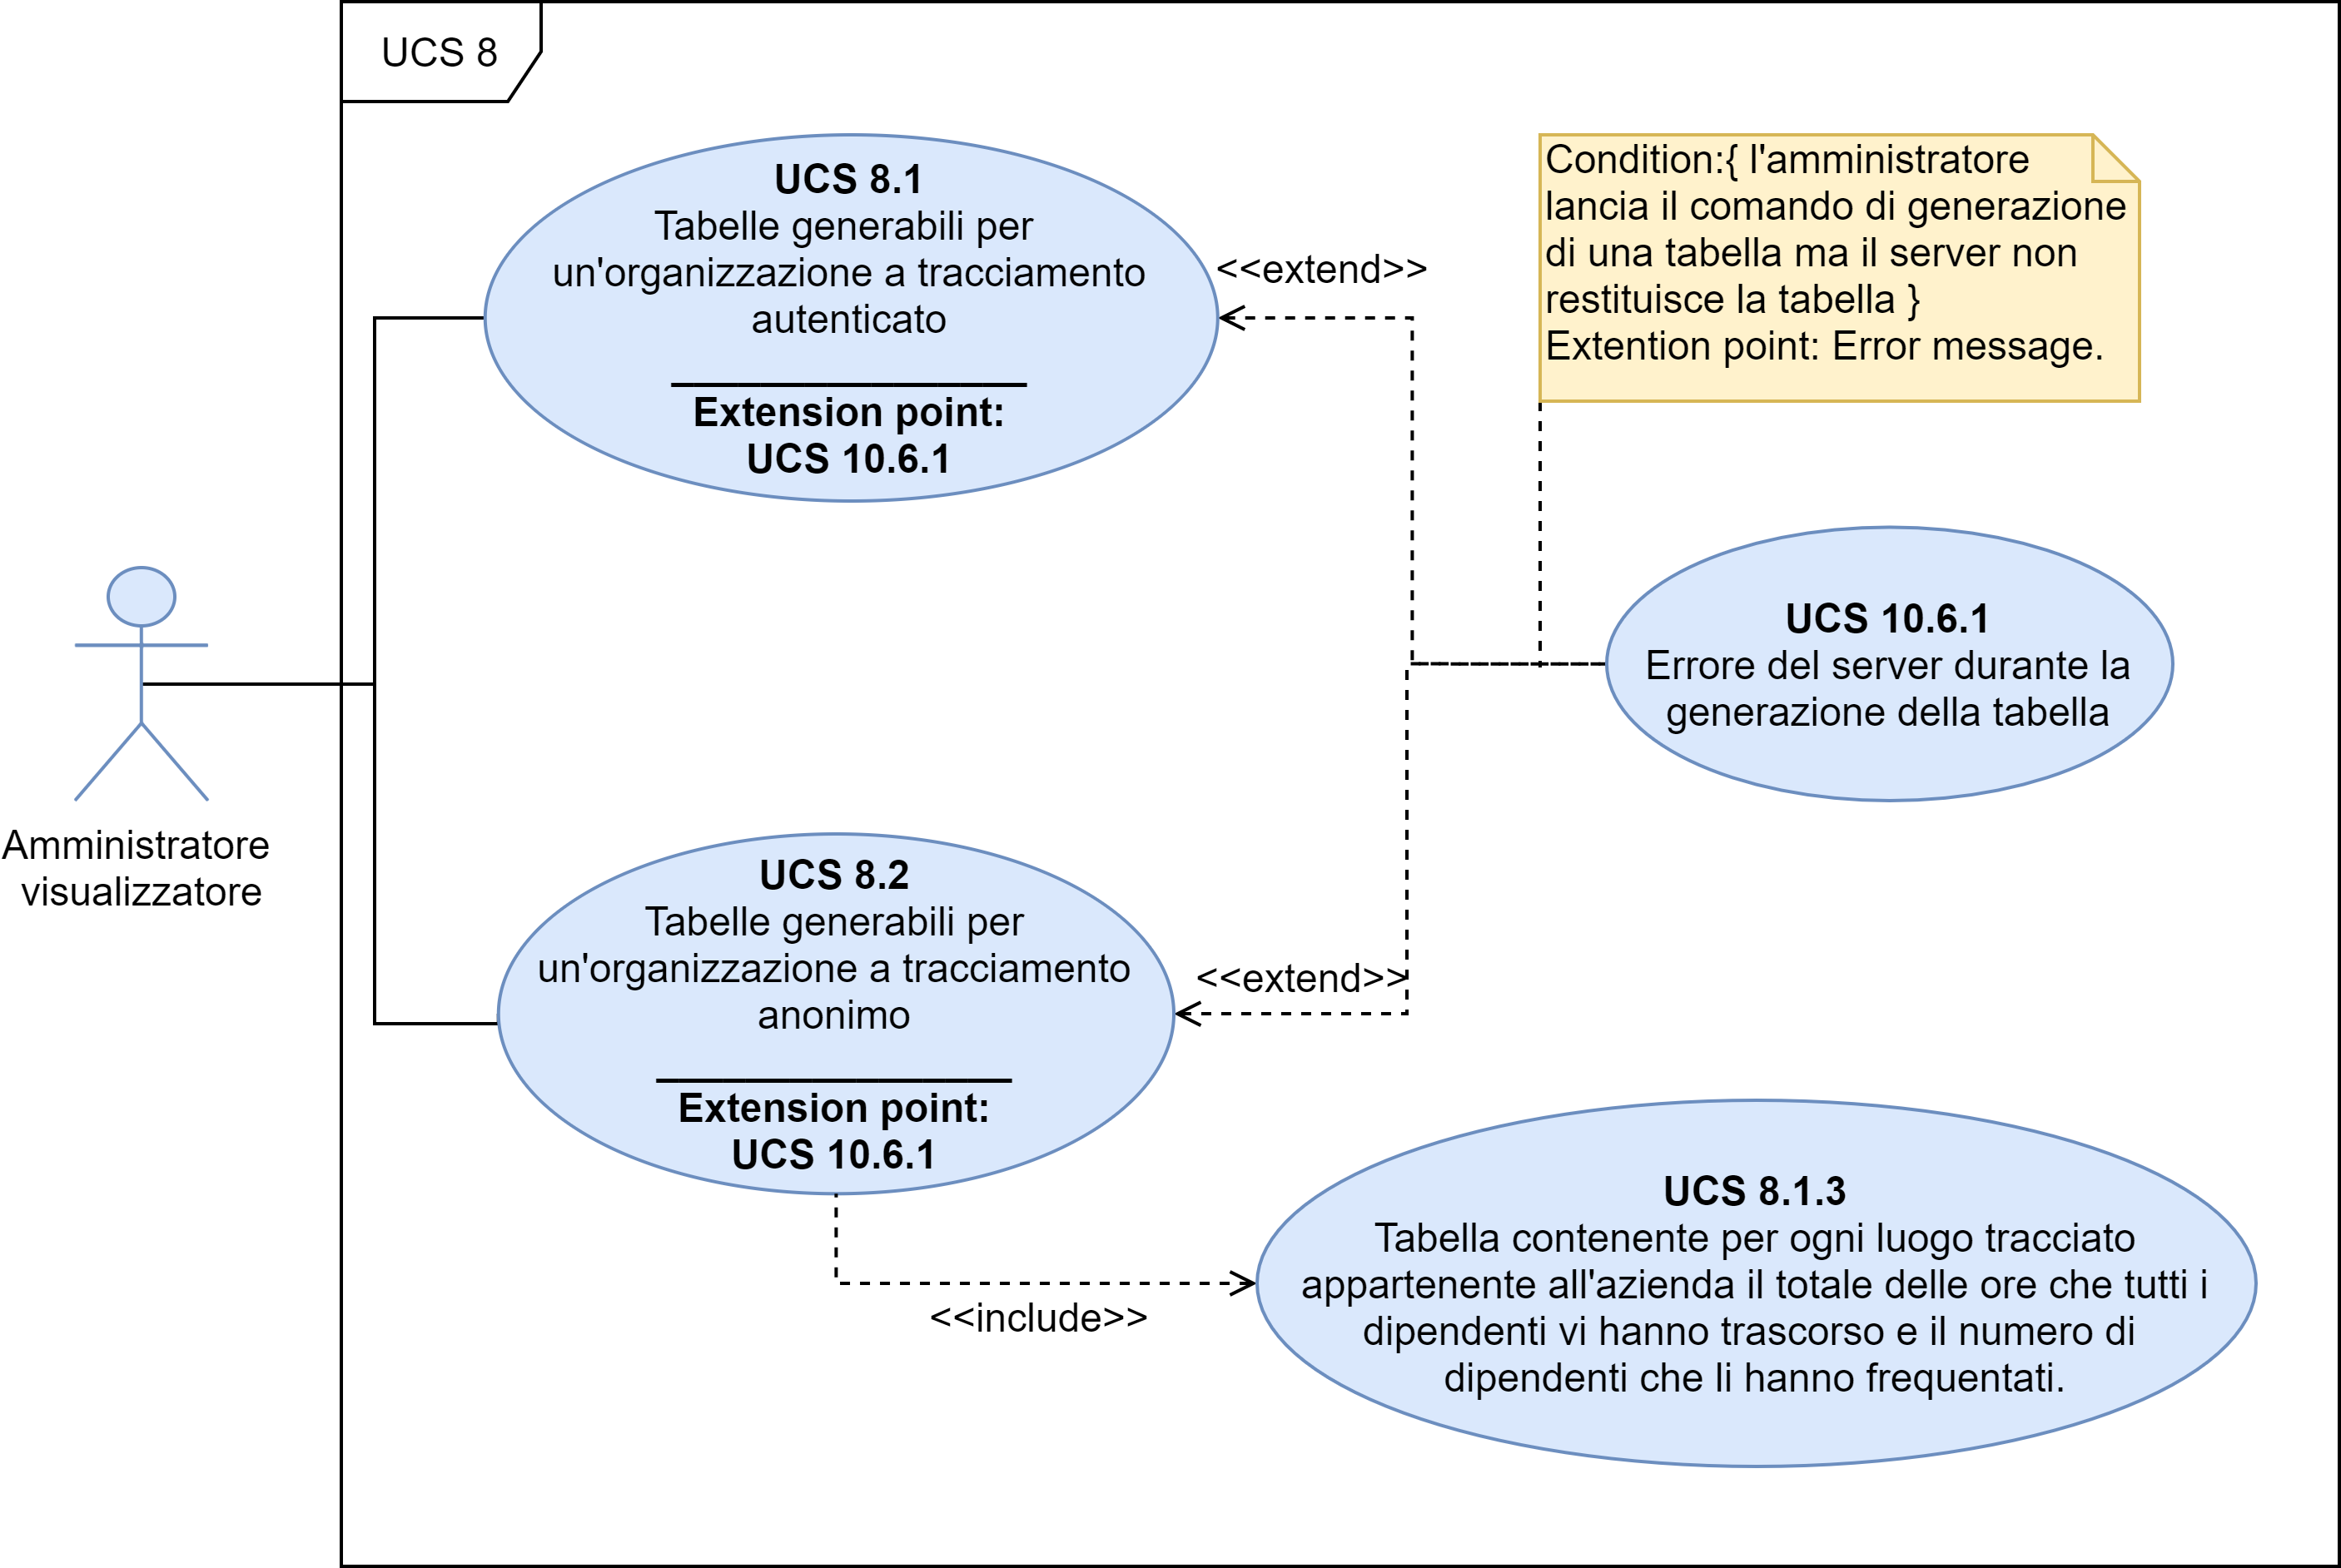
\includegraphics[scale=0.53]{Sezioni/UseCase/Immagini/UCS8.png}
    \caption{UCS 8 - Report tabellare degli accessi ai luoghi dell'organizzazione}
\end{figure}

\begin{itemize}
\item \textbf{Attori primari:} Amministratore visualizzatore
%\item \textbf{Attori secondari:}%opzionale
\item \textbf{Precondizione:} L'amministratore seleziona la funzionalità di generazione della tabella degli accessi per la sua \glo{organizzazione}.
\item \textbf{Postcondizione:} L'amministratore può visionare la tabella che è stata correttamente formata.
\item \textbf{Scenario principale:} L'amministratore autenticato si trova nella pagina della sua \glo{organizzazione} e può selezionare la funzionalità di generazione della tabella degli accessi alla sua \glo{organizzazione}, le possibilità variano in funzione della presenza di \glo{tracciamento autenticato} [UCS 8.1] oppure \glo{tracciamento anonimo} [UCS 8.2].
%\item \textbf{Inclusioni:} 
\end{itemize}

\subsubsection{UCS 8.1 - Tabelle generabili dall'amministratore di un'organizzazione a tracciamento autenticato}%sea level


\begin{itemize}
\item \textbf{Attori primari:}Amministratore visualizzatore
\item \textbf{Precondizione:} L'amministratore può scegliere tra 3 tipi di tabelle da generare.
\item \textbf{Postcondizione:} L'amministratore può visionare la tabella correttamente formata.
\item \textbf{Scenario principale:} L'amministratore seleziona un tipo di tabella tra i 3 possibili:
	\begin{itemize}%flusso di eventi
	\item Tabella contenente per ogni utente l'ora di entrata e uscita in ogni \glo{luogo} tracciato appartenente all'\glo{organizzazione} [UCS 8.1.1];
	\item Tabella contenente per ogni utente il totale delle ore spese in ogni \glo{luogo} tracciato appartenente all'\glo{organizzazione} [UCS 8.1.2];
	\item Tabella contenente per ogni \glo{luogo} tracciato appartenente all'azienda il totale delle ore che tutti i dipendenti vi hanno passato e il numero di dipendenti che li hanno frequentati [UCS 8.1.3].
\end{itemize}
Dopo la selezione la tabella viene mostrata a video e l'amministratore può quindi visionarla.
\item \textbf{Estensioni:}
	\begin{enumerate}
		\item UCS 10.6.1 - Errore del server durante la generazione della tabella.
	\end{enumerate}
%\item \textbf{Inclusioni:}
\end{itemize}

\begin{figure}[h!]
	\centering
    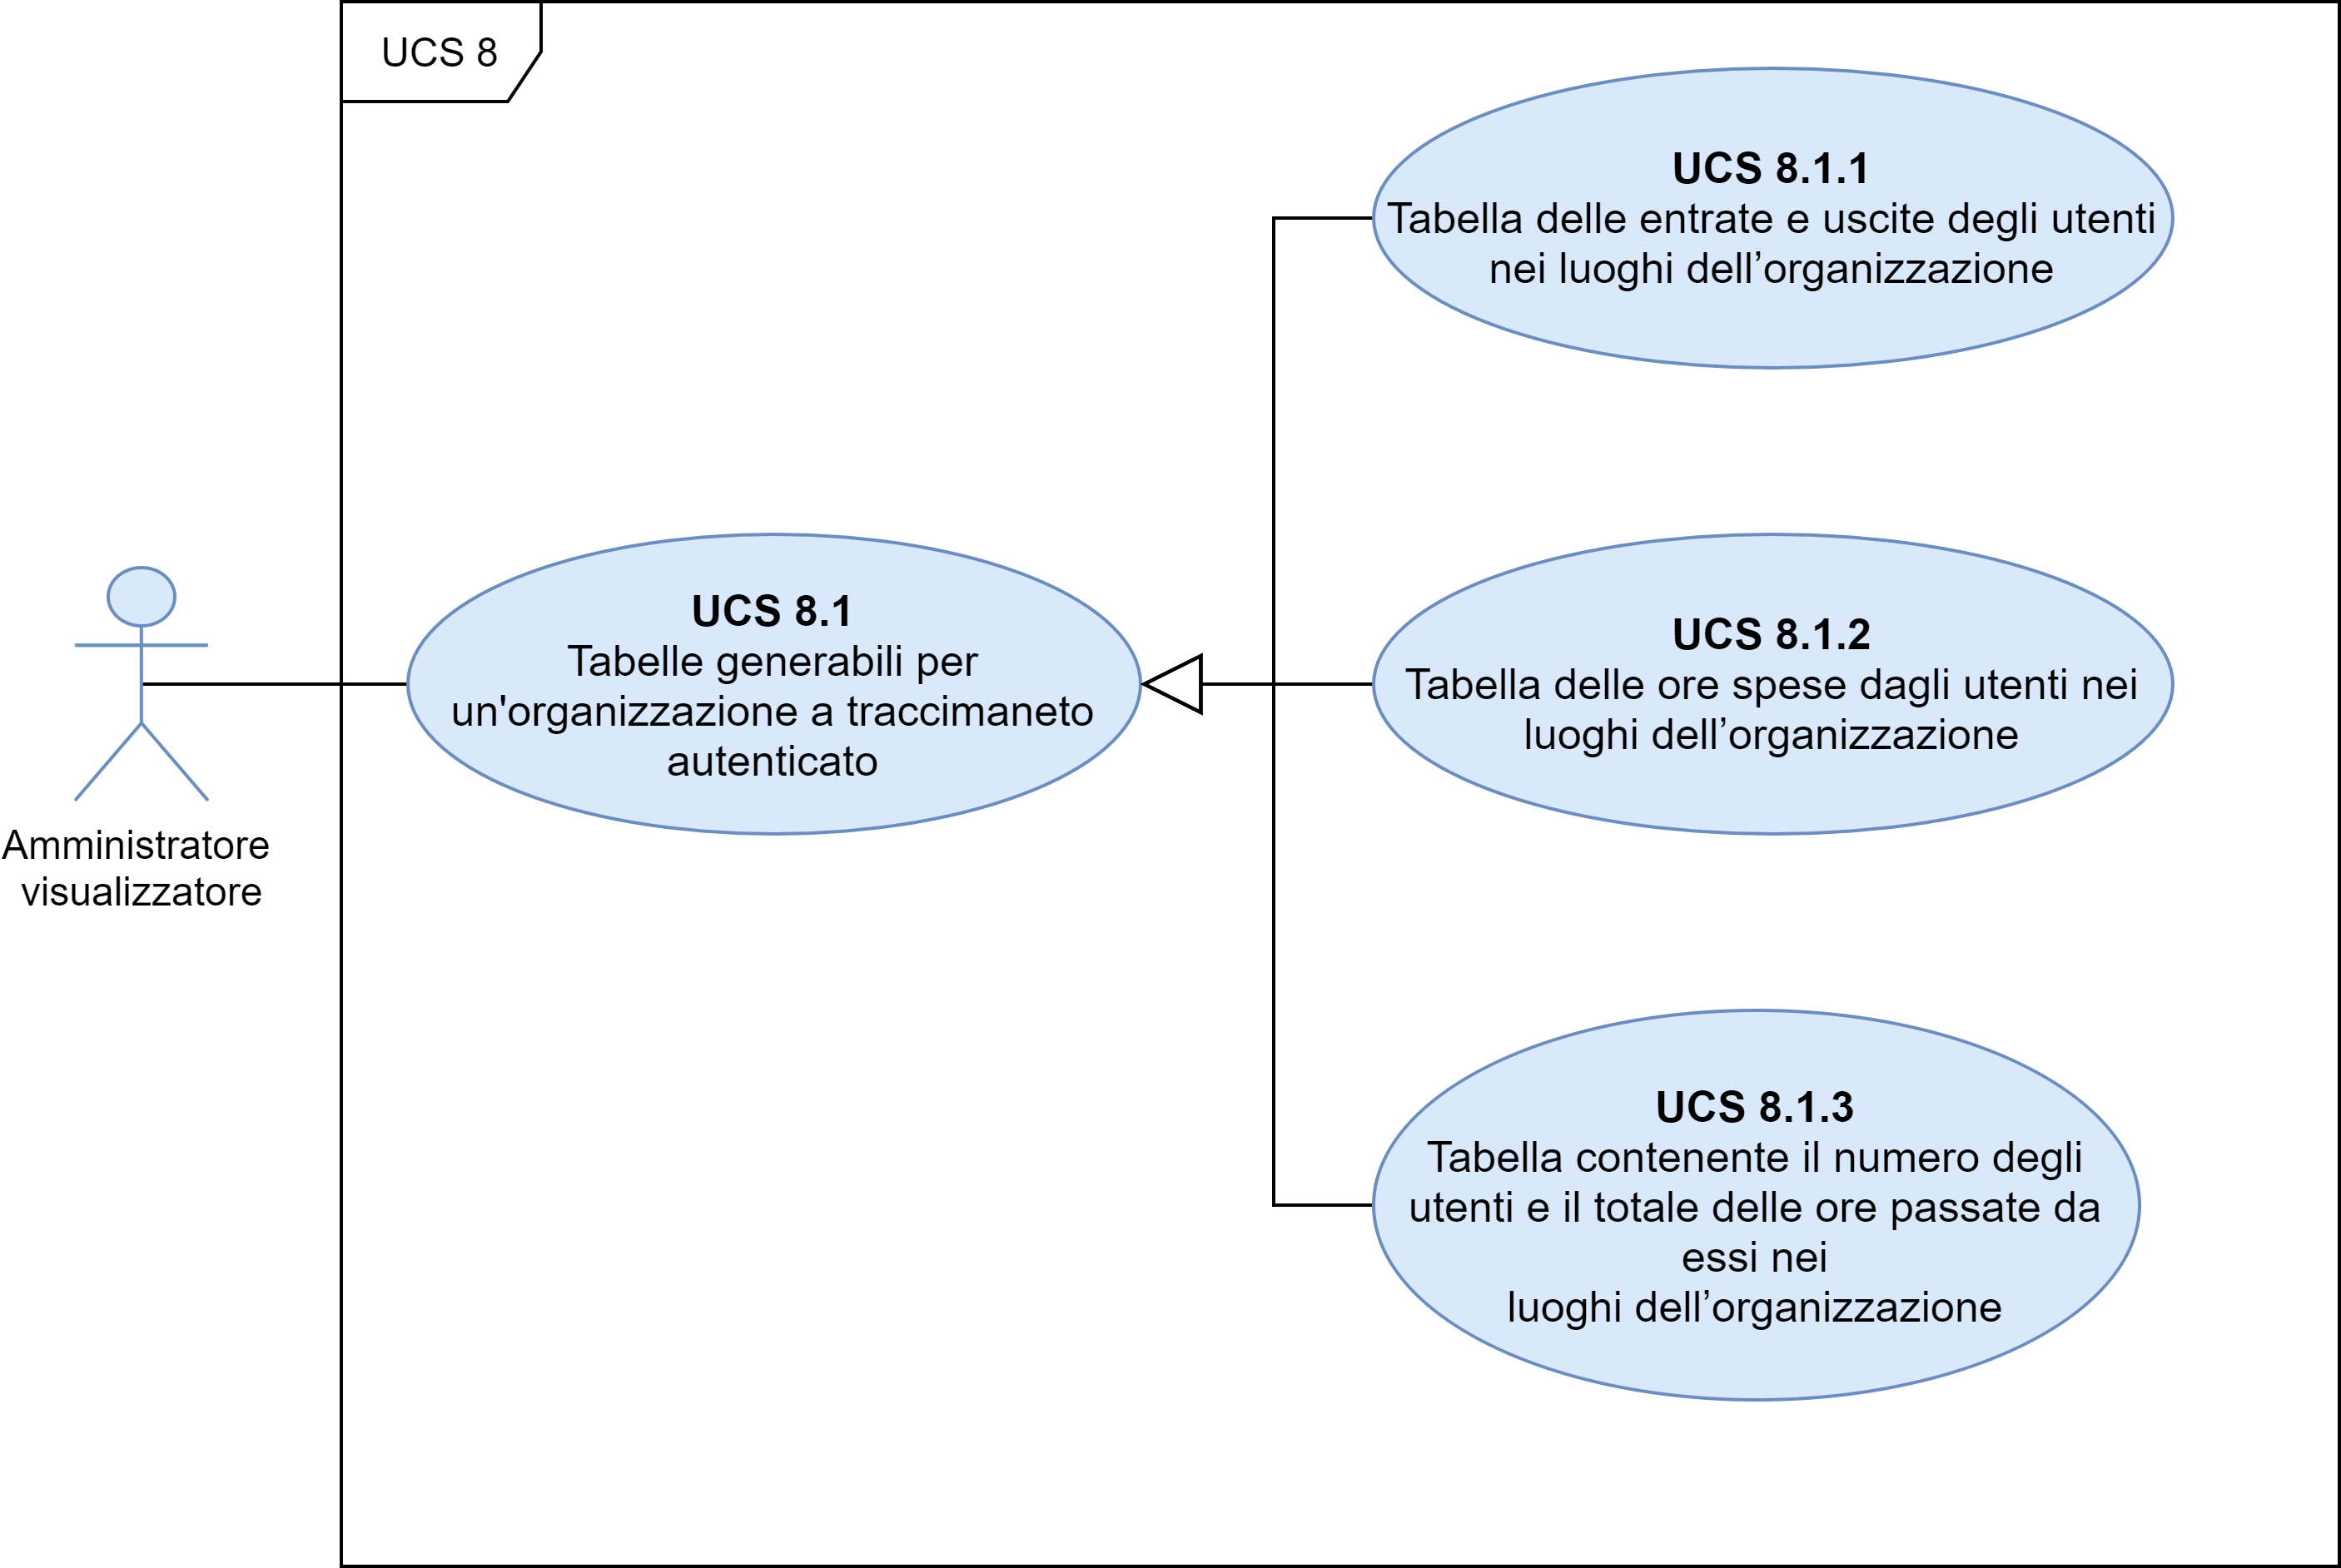
\includegraphics[scale=0.53]{Sezioni/UseCase/Immagini/UCS8.1.png}
    \caption{UCS 8.1 - Tabelle generabili dall'amministratore di un'organizzazione a tracciamento autenticato}
\end{figure}

\subsubsection{UCS 8.1.1 - Tabella delle entrate e uscite degli utenti nei luoghi dell'organizzazione}%fish level
\begin{itemize}
\item \textbf{Attori primari:} Amministratore visualizzatore
\item \textbf{Precondizione:} L'amministratore seleziona questa opzione per la generazione della tabella.
\item \textbf{Postcondizione:} La tabella richiesta è corretta e l'amministratore può visionarla.
\item \textbf{Scenario principale:} L'amministratore genera una tabella contenente per ogni utente l'ora di entrata e uscita in ogni luogo tracciato appartenente all'\glo{organizzazione}.
\item \textbf{Generalizzazione:}
	\begin{enumerate}
		\item UCS 8.1 - Tabelle generabili dall'amministratore di un'organizzazione a \glo{tracciamento autenticato}.
	\end{enumerate} 
\end{itemize}

\subsubsection{UCS 8.1.2 - Tabella delle ore spese dagli utenti nei luoghi dell'organizzazione}%fish level
\begin{itemize}
\item \textbf{Attori primari:} Amministratore visualizzatore
\item \textbf{Precondizione:} L'amministratore seleziona questa opzione per la generazione della tabella.
\item \textbf{Postcondizione:} La tabella richiesta è corretta e l'amministratore può visionarla.
\item \textbf{Scenario principale:} L'amministratore genera una tabella contenente per ogni utente il totale delle ore spese in ogni \glo{luogo} tracciato appartenente all'\glo{organizzazione}.
\item \textbf{Generalizzazione:}
	\begin{enumerate}
		\item UCS 8.1 - Tabelle generabili dall'amministratore di un'organizzazione a \glo{tracciamento autenticato}.
	\end{enumerate} 
\end{itemize}

\subsubsection{UCS 8.1.3 - Tabella contenente il numero degli utenti e il totale delle ore passate da essi nei luoghi dell'organizzazione}%fish level
\begin{itemize}
\item \textbf{Attori primari:} Amministratore visualizzatore
\item \textbf{Precondizione:} L'amministratore seleziona questa opzione per la generazione della tabella.
\item \textbf{Postcondizione:} La tabella richiesta è corretta e l'amministratore può visionarla.
\item \textbf{Scenario principale:} L'amministratore genera una tabella contenente per ogni luogo tracciato appartenente all'azienda il totale delle ore che tutti i dipendenti vi hanno passato e il numero di dipendenti che li hanno frequentati.
\item \textbf{Generalizzazione:}
	\begin{enumerate}
		\item UCS 8.1 - Tabelle generabili dall'amministratore di un'organizzazione a \glo{tracciamento autenticato}.
	\end{enumerate} 
\end{itemize}

\subsubsection{UCS 8.2 - Tabelle generabili dall'amministratore di un'organizzazione a tracciamento anonimo}%sea level
\begin{itemize}
\item \textbf{Attori primari:} Amministratore visualizzatore
\item \textbf{Precondizione:} L'amministratore seleziona la funzionalità di generazione della tabella.
\item \textbf{Postcondizione:} La tabella è stata correttamente formata e l'amministratore può visionarla.
\item \textbf{Scenario principale:} L'amministratore genera tabelle di un'organizzazione a tracciamento anonimo.
\item \textbf{Flusso di eventi:}
	\begin{enumerate}%flusso di eventi
	\item L'amministratore seleziona la funzionalità di generazione tabella;
	\item Viene creata una tabella contenente per ogni luogo dell'\glo{organizzazione} il numero di visitatori e le ore trascorse al suo interno [UCS 8.1.3];
	\item L'amministratore può visionare la tabella correttamente formata.
\end{enumerate}
\item \textbf{Inclusioni:} 
\begin{itemize}
		\item UCS 8.1.3 - Tabella contenente per ogni luogo tracciato appartenente all'azienda il totale delle ore che tutti i dipendenti vi hanno passato e il numero di dipendenti che li hanno frequentati.
	\end{itemize}
	\item \textbf{Estensioni:}
	\begin{enumerate}
		\item UCS 10.6.1 - Errore del server durante la generazione della tabella.
	\end{enumerate}
\end{itemize}
